% !TEX root = ../main.tex

% 中英标题：\chapter{中文标题}[英文标题]

\chapter{国内外研究现状及分析}
\section{国内外研究现状}
CAFA（Critical Assessment of Function Annotation）\cite{zhou2019cafa}挑战是一项在生物信息学领域极具挑战性的竞赛，其目的是评估并推动蛋白质功能预测方法的发展。这项挑战由国际生物信息学研究社区组织，并吸引了来自世界各地的研究人员参与。简而言之，CAFA 组织者提供大量的蛋白质序列，参与者需要使用他们的计算方法来预测这些蛋白质的功能，并将这些预测与实际的注释进行比较，以评估计算方法的准确性。CAFA 挑战为研究人员提供了一个平台，让他们能够评估和比较各自的蛋白质功能预测计算方法。此外，CAFA 挑战已成为生物信息学领域的一项重要竞赛，在这里，研究人员可以了解各种现有功能预测算法的优点和缺点，并促进蛋白质功能预测方法的发展。

基于多模态预训练的蛋白质功能预测是一种前沿的深度学习方法，它通过整合来自蛋白质的不同数据源,例如序列、结构和已知的功能标注来训练模型。这种方法不依赖于大量的直接训练数据，而是通过挖掘和融合多种类型的生物数据来预测蛋白质的功能。模型通过学习这些不同模态的内在联系，构建一个能够从输入特征（如氨基酸序列和三维结构）映射到其功能属性的框架。在多模态预训练中，关键的挑战是如何有效地整合来自不同数据源的信息，并捕获这些数据之间的复杂关系。

\section{国内外文献综述及简析}
\subsection{蛋白质功能预测研究现状}
在过去几十年里，国内外学者提出了许多计算方法来预测蛋白质的功能。这些方法可以根据它们所利用的信息类型分为三大类：基于序列的方法、基于3D结构的方法、基于混合信息的方法。需要注意的是，这些分类并非严格区分，它们之间存在重叠和相关性，例如一些基于结构的计算方法也会利用序列信息来预测蛋白质的功能。

(1)基于蛋白质序列的方法

基于序列的方法主要针对蛋白质序列，通过提取与功能相关的潜在特征来预测蛋白质的功能。这些方法更深入地研究氨基酸序列中包含的信息，并试图捕捉与嵌入其中的蛋白质功能相关的细微特征。

BLAST\cite{altschul1990basic}是一种广泛使用的工具，用于搜索数据库，寻找与目标蛋白相似的序列，从而推断目标蛋白的潜在功能。然而单纯依靠序列比对工具预测蛋白质功能的准确性不高，因此许多方法已经开始结合神经网络。结合卷积神经网络的预测结果，DeepGOPlus\cite{kulmanov2020deepgoplus}通过搜索已知功能的相似蛋白来提高预测精度。与之前的模型DeepGO\cite{kulmanov2018deepgo}相比，DeepGOPlus在去除PPI特征的同时提高了预测性能。此外它克服了序列长度的限制，用单热编码取代了氨基酸三元组嵌入层。HiFun\cite{wu2023hifun}从蛋白质可以表示为一种语言的想法中获得灵感，使用BLOSUM62矩阵\cite{song2014parameterized}和FastText嵌入蛋白质序列。基于BLOSUM62矩阵的向量被馈送到卷积层以提取潜在特征，而基于FastText嵌入的矩阵被馈送到由卷积神经网络(CNN)和具有自关注架构的双向长短期记忆(BiLSTM)\cite{xu2019sentiment}组成的架构中。从CNN中提取的特征向量被传递到BiLSTM的两个隐藏层，这两个隐藏层利用前后的上下文信息来增强特征表示。此外，HiFun对BiLSTM层的输出执行自关注机制，以估计氨基酸的重要性。

这些方法仅利用蛋白质序列进行蛋白质功能预测，在发现新蛋白质的功能方面发挥着重要作用。通过研究实验表明，依赖于蛋白质序列的方法可以显著提高功能类别中MFO的预测。然而许多蛋白质在功能上相似，但在序列上不同，这可能导致对序列相似性低的蛋白质的预测性能较差。

(2)基于蛋白质结构的方法

基于三维结构的方法侧重于蛋白质的结构特征，蛋白质结构经常被翻译成接触图，从中捕获与功能密切相关的特征。在这些方法中，蛋白质序列经常被用作输入特征之一，对于功能主要受结构特征影响的蛋白质，基于三维结构的方法具有更明显的优势。

DeepFRI\cite{gligorijevic2021structure}将图卷积网络(GCN)作为其核心技术，首先利用蛋白质家族数据库(Pfam)\cite{mistry2021pfam}中的序列对具有长短期记忆的语言模型(LSTM-LM)\cite{graves2012long}进行预训练，提取序列的残差特征；其次它将蛋白质结构转化为接触图，两者都用作GCN的输入。LSTM-LM从序列中学习的特征和GCN从接触图中学习的特征显著提高了蛋白质功能预测的性能。HEAL\cite{gu2023hierarchical}与DeepFRI进行了比较，作者首先使用蛋白质数据库(Protein Data Bank, PDB)中的蛋白质训练模型heal-PDB，该模型的性能与DeepFRI相当。通过加入AlphaFold2\cite{varadi2022alphafold}预测的蛋白质结构，HEAL的性能得到了显著提高。HEAL首先基于序列节点特征和接触图为每个蛋白质构建图，并将其输入到由消息传递神经网络和分层图转换器组成的架构中，然后使用监督学习和比较学习来优化网络。Struct2GO\cite{jiao2023struct2go}同时接受序列和结构信息作为输入，利用SeqVec模型\cite{heinzinger2019modeling}提取序列特征，利用基于自关注机制的分层图池化模型从AlphaFold2预测的结构中提取特征。为了最大限度地利用结构信息，Struct2GO采用Node2vec\cite{grover2016node2vec}算法在蛋白质结构网络中生成氨基酸级嵌入。这些嵌入被用作图池模型的初始节点特征。与实验确定的蛋白质结构相比，AlphaFold2提供了丰富的高分辨率结构信息，显著提高了模型预测精度。

\begin{figure}[h]
\centering
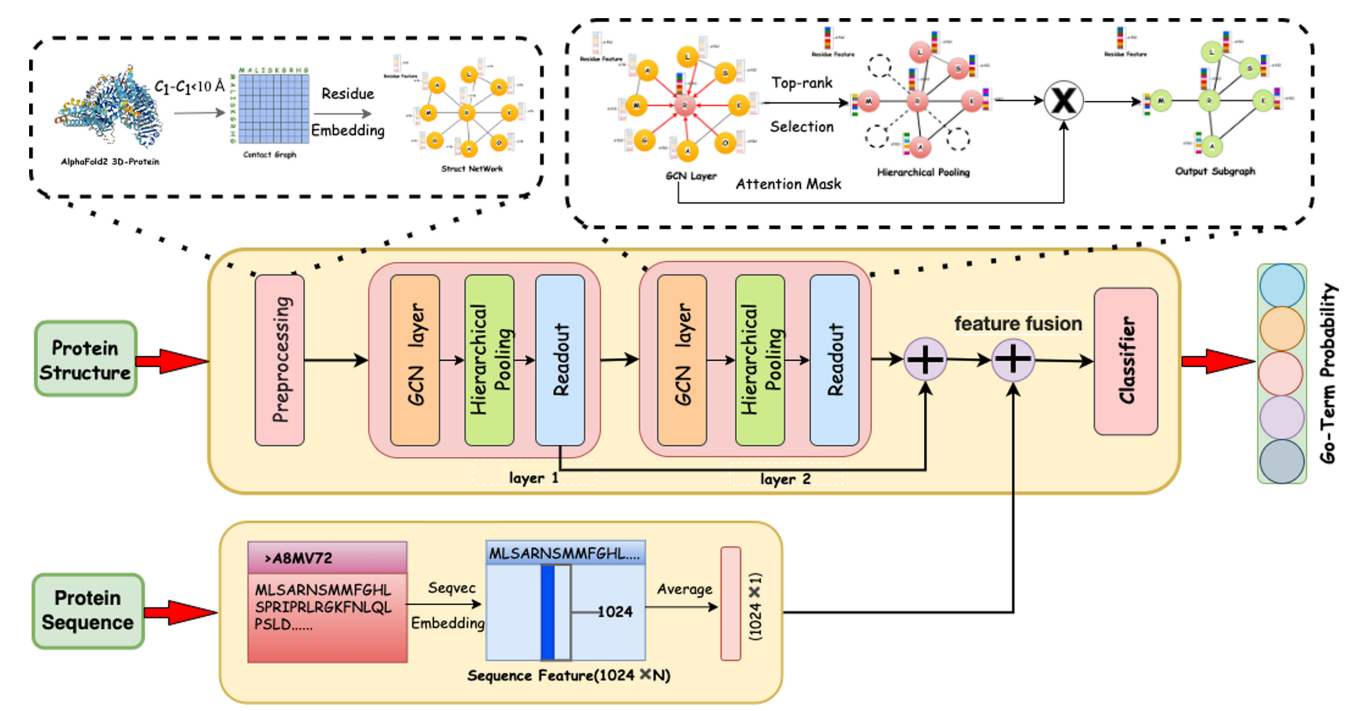
\includegraphics[width = 1\textwidth]{figures/图片2.png}
\caption{Struct2GO模型图\cite{jiao2023struct2go}}
\label{fig:strct2go}
\end{figure}

这些方法将蛋白质结构与蛋白质序列结合起来，大大提高了蛋白质功能预测的准确性。对于高相似性的蛋白质，仅使用序列特征很难区分细微的功能差异，结合结构特征可以帮助克服这一问题。这种方法的缺点是它们只关注蛋白质的结构特征，而忽略了蛋白质之间的相互作用。

（3）基于混合信息的方法

基于混合信息的方法强调各种信息类型的组合，如蛋白质序列、蛋白质结构、PPI网络或InterPro特征等的整合方法。CAFA挑战表明，有效整合不同的信息类型可以真正提高蛋白质功能预测的准确性，目前混合信息是该领域发展的主要趋势。

DeepGraphGO\cite{you2021deepgraphgo}是一种基于多物种图神经网络的方法。首先利用InterProScan\cite{jones2014interproscan}工具生成蛋白质的InterPro特征向量，并结合PPI网络将InterPro特征向量作为网络中的节点特征，然后通过多个图卷积层捕获网络中的高阶信息。此外，DeepGraphGO的优势在于它采用了多物种策略，利用所有物种的蛋白质数据来训练单个模型，不仅节省了时间和计算资源，而且提高了模型的泛化能力。DeepGOZero\cite{kulmanov2022deepgozero}使用InterPro的二进制特征作为输入，并通过两个多层感知器（MLP）层生成稠密特征。最显著的是DeepGOZero可以利用基因本体（GO)形式公理通过零样本学习来预测新功能，这些GO形式公理通过EL Embedding\cite{kulmanov2019embeddings}表示为n球体的类嵌入到几何模型的向量关系中来表示本体语义。DeepGOZero将模型理论与神经网络结合起来预测蛋白质功能，具体来说它计算预测结果和标签之间的二进制交叉熵损失，然后通过EL Embedding指定的本体公理派生的损失来优化它们。此外DeepGOZero 还整合了同源蛋白的相似性信息，以进一步增强预测性能。DeepGO-SE\cite{kulmanov2024protein}对DeepGOZero进行了一系列改进,它通过使用预训练的大型蛋白质语言模型结合神经符号模型来预测蛋白质序列的功能，该神经符号模型将功能预测视为近似语义蕴涵。作者使用ESM2\cite{lin2023evolutionary}蛋白质语言模型来生成单个蛋白质的表示，与DeepGOZero类似，将ESM2嵌入投射到由GO公理生成的嵌入空间（EL Embeddings）中。与DeepGOZero不同的是，作者使用这些世界模型来执行“语义蕴涵”：当且仅当在所有使理论T为真的世界模型中，陈述$\varphi$也为真时，$\varphi$才由理论T蕴涵 ($T\vDash\varphi$)\cite{zadeh1975concept}。利用这种近似语义蕴涵的形式，作者展示了GO扩展版本中的公理可以增强分子功能的预测。此外作者通过整合有关有机体蛋白质相互作用网络改进了复杂生物过程和细胞成分的预测。

\begin{figure}[h]
\centering
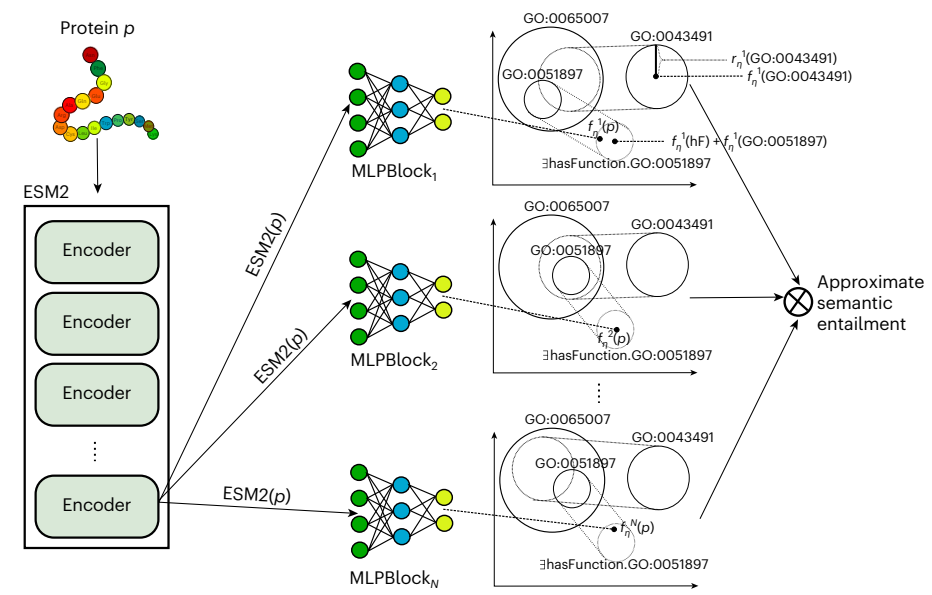
\includegraphics[width = 1\textwidth]{figures/图片5.png}
\caption{DeepGO-SE模型图\cite{kulmanov2024protein}}
\label{fig:deepgose}
\end{figure}

\FloatBarrier

这些方法通过有效地融合来自多个来源的信息，从多个方面捕捉蛋白质的多样性特征，从而提高功能预测的性能。然而融合来自不同数据源的信息通常需要更复杂的算法或技术来提取特征，特别是在大规模数据集上，这可能导致计算资源和时间的消耗增加。此外，一些蛋白质可能缺乏某些特征的来源信息，导致缺乏这些蛋白质的全面融合信息，因此正确处理缺失数据是此类方法的主要挑战。

\subsection{多模态预训练蛋白质功能预测研究现状}
多模态预训练技术通过整合多种生物信息数据，如蛋白质序列、结构和已有的功能标注，克服了传统单一数据源预训练模型在自动功能预测（AFP）领域的局限性。这种方法的核心优势在于能够利用来自不同生物学模态的信息，提高预测未标注或罕见功能的准确性。在多模态预训练中，模型不仅学习从序列或结构直接推断功能的能力，还能通过整合这些不同模态的信息来获得更深层次的生物学见解。

CFAGO\cite{wu2023cfago}基于多头注意机制在两个阶段交叉融合PPI网络和蛋白质属性\cite{vaswani2017attention}。第一步是预训练，其中使用自编码器来学习PPI网络和蛋白质属性中的隐藏特征，
自动编码器具有忽略数据中的噪声的能力。第二步是微调，将预训练好的编码器与两层全连接神经网络相结合，预测蛋白质功能。消融实验表明，与注意机制相比，预训练对成绩提高的作用更大。

\begin{figure}[h]
\centering
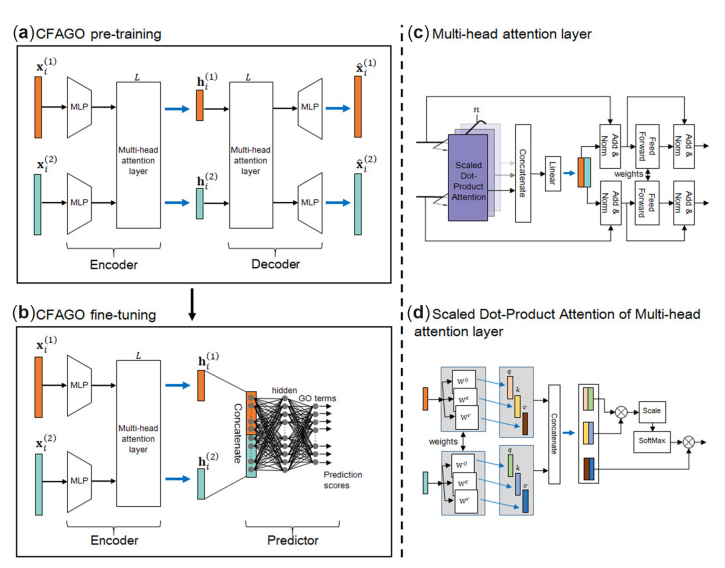
\includegraphics[width = 1\textwidth]{figures/图片3.png}
\caption{CFAGO模型图\cite{wu2023cfago}}
\label{fig:cfago}
\end{figure}

MASSA\cite{hu2023multimodal}构建了一个新型深度学习框架，用于整合蛋白质序列、结构和功能注释的多模态数据。MASSA通过设计与蛋白质生物学理解相符的特定任务预训练目标，在多任务学习过程中提取详细的蛋白质域特征，从而在蛋白质属性、蛋白质-蛋白质相互作用和蛋白质-配体相互作用等各种下游任务中增强性能。研究表明，该框架在特定下游任务中实现了最先进的结果，并引入了一种新的基于最优传输的度量来量化从预训练模型到不同下游任务的转移性，有效地展示了整合多种类型蛋白质数据的优势，为计算生物学和生物信息学的发展提供了新的视角。

\begin{figure}[h]
\centering
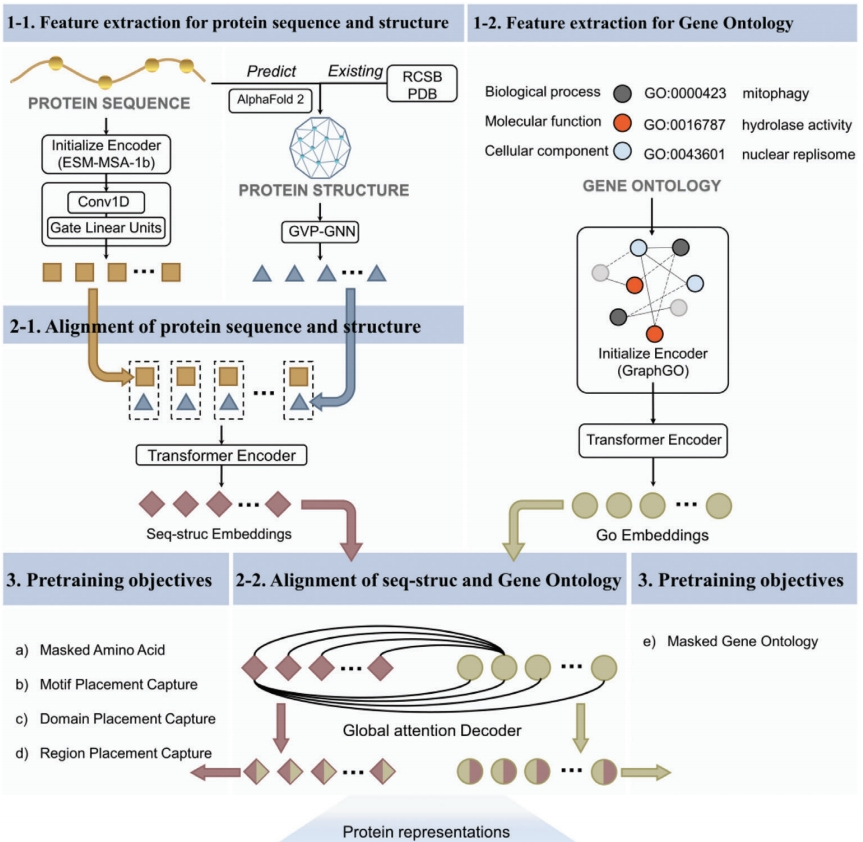
\includegraphics[width = 1\textwidth]{figures/massa.png}
\caption{MASSA模型图\cite{hu2023multimodal}}
\label{fig:massa}
\end{figure}

\subsection{扩散模型分类器研究现状}
最近大规模的文本到图像扩散模型显著提升了基于文本生成图像的能力，这些模型可以根据各种提示生成逼真的图像，并表现出强大的组合泛化能力。虽然到目前为止，大多数使用案例都集中在图像生成上，但扩散模型还可以提供条件密度估计，这对于图像生成之外的任务也很有用。国内外已有不少学者利用扩散模型进行零样本分类，并取得了不错的性能结果。

Kevin Clark与Priyank Jaini\cite{clark2024text}提出文本到图像的扩散模型是零样本分类器，其关键思想是利用扩散模型的能力，在给定标签的文本描述的情况下，将带有噪声的图像去噪，作为该标签可能性的代理。模型以原始图像 \(x_0\) 作为输入，生成一个加噪的图像 \(x_t\)，这是通过在扩散模型中加入噪声来实现的。使用不同的标签提示（如“Cat”、“Horse”、“Frog”等），扩散模型条件化这些标签提示，以去噪输入图像。在每个时间步$t$上，扩散模型输出与这些标签相关的去噪图像,对每个标签提示在不同时间步的去噪图像计算得分,通过计算得分最小的标签来确定最终的分类结果。

\begin{figure}[h]
\centering
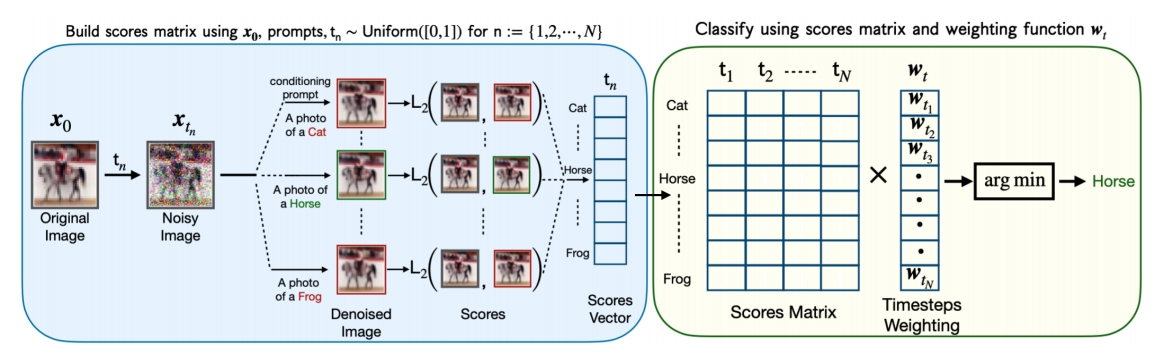
\includegraphics[width = 1\textwidth]{figures/noise.png}
\caption{使用扩散模型进行零样本分类模型图\cite{clark2024text}}
\label{fig:texttoimage}
\end{figure}

\FloatBarrier

Alexander Li等人\cite{li2023your}证明了大规模文本到图像扩散模型(如Stable diffusion\cite{rombach2022high})的密度估计可以用于执行零样本分类，而无需任何额外的训练。其中输入图像被加噪后，通过扩散模型和文本条件来去噪，并计算每个条件下的损失，最终模型选择那个最能准确预测噪声的条件（即损失最小的条件）作为分类结果。输入的文本条件 \(c\) 是与类别相关的描述（如 a photo of a [class name]），这是模型用来指导分类的提示。模型的分类目标是找到最佳的文本条件 \(c\)，使得在所有时间步 \(t\) 中，模型预测的噪声 \(\hat{\epsilon}\) 最接近实际添加的噪声 \(\epsilon\)。Chen等人\cite{chen2023robust}提出了鲁棒扩散分类器(Robust diffusion Classifier, RDC)，这是一种由预训练的扩散模型构建的生成分类器，具有对抗鲁棒性。RDC首先最大化给定输入的数据似然，然后使用扩散模型通过贝叶斯定理估计的条件似然来预测优化后输入的类概率。具体过程为给定输入图像 \(x\)，首先通过一个扩散模型对其进行处理，通过迭代优化来最大化图像的似然估计。这个过程涉及到多个时间步 \(t\) 的迭代，从而使优化后的图像 \(x_t\) 更符合扩散模型的概率分布。优化目标是最小化噪声预测误差（即扩散损失），这个误差在每个时间步 \(t\) 上进行平均。然后对优化后的图像 \(x_t\) 使用扩散模型再次进行处理，以估计每个类别 \(y\) 的条件对数似然 \(\log p_\theta(x \mid y_k)\)。通过贝叶斯定理，计算每个类别的概率 \(p(y \mid x)\)，并最终选择具有最大概率的类别作为预测结果。

\subsection{蛋白质功能预测领域研究进展总结}
综上所述，蛋白质功能预测领域在国内外取得了显著进展，主要包括基于序列、结构以及多模态信息的方法。CAFA挑战作为评估和推动蛋白质功能预测的重要平台，显示了不同方法的优势和不足。基于序列的方法通过捕捉氨基酸序列中的特征实现预测，但在处理序列相似性低的蛋白质时存在局限。基于结构的方法通过分析蛋白质的三维特征来提高预测准确性，特别是在结合图神经网络时取得了优异的性能。然而，基于接触图提取结构特征的方法在计算资源上面临诸多限制。多模态预训练技术通过整合序列、结构和蛋白质功能注释等多种数据来源，进一步提升了模型的准确性和泛化能力，但也面临数据融合复杂性和计算资源需求增加的问题。此外，扩散模型在零样本分类中的应用展示了其在蛋白质功能预测领域的潜力。本课题将继续探索这些方法的优化和扩展，特别是在高维和复杂数据的处理上，进一步提升蛋白质功能预测的性能和应用范围。